\section{Задача классификации}
Задачи классификации --- это задачи, в которых объект должен быть отнесен к одному из $n$ классов на основе индекса сходства его характеристик с каждым классом. Под классами понимается набор подобных объектов. Объекты считаются похожими на основе совпадающих характеристик, таких как цвет, форма, размер и т.д. Классы определяются на основе их уникальных меток. В частности, задача  <<распознавания действий человека за рулем автомобиля по фото>>  является задачей классификации.

Для решения задачи классификации используются такие методы как:

\begin{itemize}[leftmargin=1.6\parindent, label*=---]
	\item методы на основе глубокого обучения;
	\item методы основанные на экземплярах;
	\item методы на основе деревьев принятия решений.
\end{itemize}

\section{Обзор методов классификации}

\subsection{Методы на основе глубокого обучения}

Методы на основе глубокого обучения представляют собой один из подходов для решения задачи классификации изображений. Они основаны на использовании глубоких нейронных сетей.

С точки зрения классификации изображений наиболее эффективным методом являются сверточные нейронные сети (CNN)\cite{cnn}. Их способность работать непосредственно с пикселями изображения позволяет извлекать сложные признаки на разных уровнях абстракции, что делает их хорошо подходящими для большинства задач классификации изображений. Кроме того, многократное применение сверток и слоев пулинга позволяет CNN эффективно обрабатывать изображения различных размеров.
\newpage

Общий алгоритм сверточных нейронных сетей включает в себя несколько ключевых этапов.


\begin{enumerate}
	\item Сверточный слой. Входные данные подвергаются свертке с несколькими
	фильтрами для извлечения различных признаков. Каждый фильтр обнаруживает определенные
	характеристики, такие как края, углы и текстуры. Это позволяет сети
	автоматически изучать различные уровни абстракции в изображениях.
	
	\item $Pooling$ слой. После каждого сверточного слоя обычно следует
	$pooling$ слой, который уменьшает размер признаковых карт, сохраняя
	наиболее важные признаки. Это способствует снижению количества параметров и
	вычислительную сложность модели, а также увеличивает инвариантность к
	масштабированию и смещению объектов на изображении.
	
	\item Полносвязанный слой. После нескольких сверточных слоев и слоев пулинга,
	выходы подаются на полносвязные слои, которые выполняют классификацию на
	основе полученных признаков.
	
	\item Функция активации. Между слоями нейронов используется функция
	активации, например ReLU (Rectified Linear Unit)\cite{relu}, которая добавляет
	не-\\линейность к модели.
	
	\item Обучение. Все параметры (веса и смещения) в сети обучаются с
	использованием методов градиентного спуска\cite{gradient-descent} и обратного
	распространения ошибки\cite{backpropagation} на больших объемах
	размеченных данных.
\end{enumerate}

\newpage

Преимущества методов на основе глубокого обучения.
\begin{itemize}[leftmargin=1.6\parindent]
	\item[1)] Автоматическое извлечение признаков без необходимости ручной настройки алгоритмов.
	\item[2)] Глубокие нейронные сети обладают способностью моделировать сложные зависимости между пикселями изображения и их классификацией.
	\item[3)]Высокая точность классификации: методы на основе глубокого обучения  достигают высоких показателей точности в классификации изображений, особенно при использовании больших наборов данных и правильной настройке гиперпараметров модели.
\end{itemize}


Однако методы на основе глубокого обучения также имеют некоторые ограничения:

\begin{itemize}[leftmargin=1.6\parindent, label*=---]
	\item требовательность к вычислительным ресурсам;
	\item необходимость большого количества размеченных данных;
	\item общность модели, некорректные экземпляры в наборе обучающих данных могут привести в переобучению.
\end{itemize}

\subsection{Методы основанные на экземплярах}

Методы основанные на экземплярах представляют собой один из подходов решения задачи классификации. Данный подход предполагает, что похожие входные данные приводят к похожим результатам, что является важным предположением для классификации. Наиболее распространенные примеры методов основанных на экземплярах -- это k-ближайших соседей (k-Nearest Neighbors, KNN) и метод опорных векторов (Support Vector Machines, SVM).

\subsubsection*{Метод опорных векторов}

Метод опорных векторов является одним из наиболее распространенных методов классификации и регрессии. Он основан на идее нахождения гиперплоскости максимальной ширины, разделяющей два класса данных. SVM может быть применен для решения задач как бинарной, так и многоклассовой классификации. На рисунке \ref{fig:svm} представлена визуализация алгоритма SVM.

\newpage

\begin{figure}[hbtp]
	\centering
	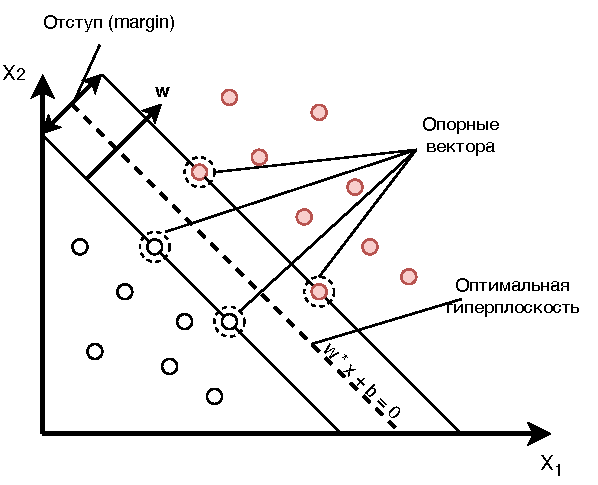
\includegraphics[width=\textwidth]{img/svm.pdf}
	\caption{Визуализация алгоритма SVM.}
	\label{fig:svm}
\end{figure}



SVM оперирует в многомерном пространстве данных, где каждое изображение представлено в виде вектора признаков. Основной шаг в методе SVM -- это построение оптимальной разделяющей гиперплоскости. Этот процесс сводится к решению оптимизационной задачи с целью максимизации отступа \\(margin) между обучающими объектами и разделяющей гиперплоскостью.

Уравнение гиперплоскости в пространстве можно представить формулой
\begin{equation}
	\label{eq:svm-line}
	w^{T}x+b=0.
\end{equation}
\eqexplSetIntro{где}
\begin{eqexpl}[15mm]
	\item{$w$} вектор нормали к гиперплоскости;
	\item{$x$} точка;
	\item{$b$} смещение.
\end{eqexpl}

Расстояние от точки $x$ до гиперплоскости  рассчитывается формулой 
\begin{equation}
	\label{eq:svm-dist}
	d=\frac{|w^Tx+b|}{|w|}.
\end{equation}

Отступ(margin) равен расстоянию между двумя параллельными плоскостями, проходящими через опорные вектора, его можно рассчитать как разницу расстояний двух опорных векторов до гиперплоскости.

Цель состоит в том, чтобы найти оптимальные значения $w$ и $b$, которые определяют гиперплоскость, удовлетворяя при этом определенным ограничениям. Запас должен быть максимальным, что означает минимизацию величины $w$.

В силу того, что весь процесс нахождения гиперплоскости сводится к нахождению скалярных произведений векторов, переход к размерности большей чем 2 осуществляется путем замены скалярного произведения на так называемое ядро -- функцию, которая является скалярным произведением в пространстве текущей размерности.

Вектор признаков для SVM обычно получается путем извлечения характеристик изображений. Эти характеристики могут включать в себя различные аспекты изображения, такие как цветовые гистограммы, текстурные дескрипторы, угловые точки или другие характеристики, которые могут быть выделены в процессе предобработки изображений.

Например, можно использовать методы извлечения признаков, такие как гистограммы направленных градиентов (HOG), которые описывают распределение градиентов яркости в изображении.

Рассмотренный метод имеет ряд преимуществ и недостатков при решении задачи классификации изображений.

Преимущества:
\begin{itemize}[leftmargin=1.6\parindent, label*=---]
	\item высокая способность обобщения;
	\item устойчивость к переобучению;
	\item возможность работы с небольшими наборами данных.
\end{itemize}

Недостатки:
\begin{itemize}[leftmargin=1.6\parindent, label*=---]
	\item требует сбора признаков;
	\item высокая вычислительная сложность в случае большого количества признаков;
	\item чувствительность к масштабированию признаков.
\end{itemize}


\subsubsection*{Метод k-ближайших соседей}
Метод k-ближайших соседей(KNN) применяется для решения задач классификации и регрессии, при этом, он основан на предпосылке о том, что близкие объекты более вероятно принадлежат к одному классу.

Последовательность действий алгоритма KNN.
\begin{itemize}[leftmargin=1.6\parindent]
	\item[1.] Определение параметра $k$,  который представляет собой число ближайших соседей, которые будут учитываться при определении класса для нового объекта.
	\item[2.] Рассчет расстояния от нового объекта до всех остальных в обучающем наборе. Это расстояние может быть рассчитано разными способами, зачастую используется евклидово расстояние\cite{eu-distance} или манхэттенское расстояние\cite{ma-distance}.
	\item[3.] Сортировка обучающего набора по возрастанию расстояния до нового объекта.
	\item[4.] Выбор первых $k$ объектов из отсортированного набора. Класс объекта определяется на основе большинства классов этих $k$ соседей.
\end{itemize}

При очень маленьком $k$ модель может стать чрезмерно чувствительной к шумам в данных, при слишком большом $k$ -- классификация может <<смазываться>> .

Важным шагом также является правильный выбор метрики расстояния, которая может значительно влиять на результаты классификации.

Для классификации изображений этим методом нужно преобразовать\\ изображение в числовой вектор. Обработка большого количества изображений может потребовать большое количество вычислительных ресурсов и времени.

% \subsubsection{Метод выделения гистограммы направленных градиентов (Histogram of Oriented Gradients, HOG).}

% Метод выделения гистограммы направленных градиентов основан на использовании локальных текстурных и геометрических свойств изображений для распознавания объектов. Он может быть использован для детекции и классификации объектов в изображениях.

% Основная идея метода HOG заключается в определении направления и силы градиентов изображения. Для каждого пикселя вычисляются градиенты в горизонтальном и вертикальном направлениях, а затем эти данные используются для создания гистограммы направленных градиентов. Гистограммы позволяют захватить информацию о текстуре и форме объекта, игнорируя незначительные детали. Затем эти гистограммы могут быть использованы для классификации объектов с помощью методов машинного обучения, таких как метод опорных векторов.

% На рисунке \ref{fig:hog} представлена схема алгоритма выделения гистограммы направленных градиентов.

% \begin{figure}[hbtp]
% 	\centering
% 	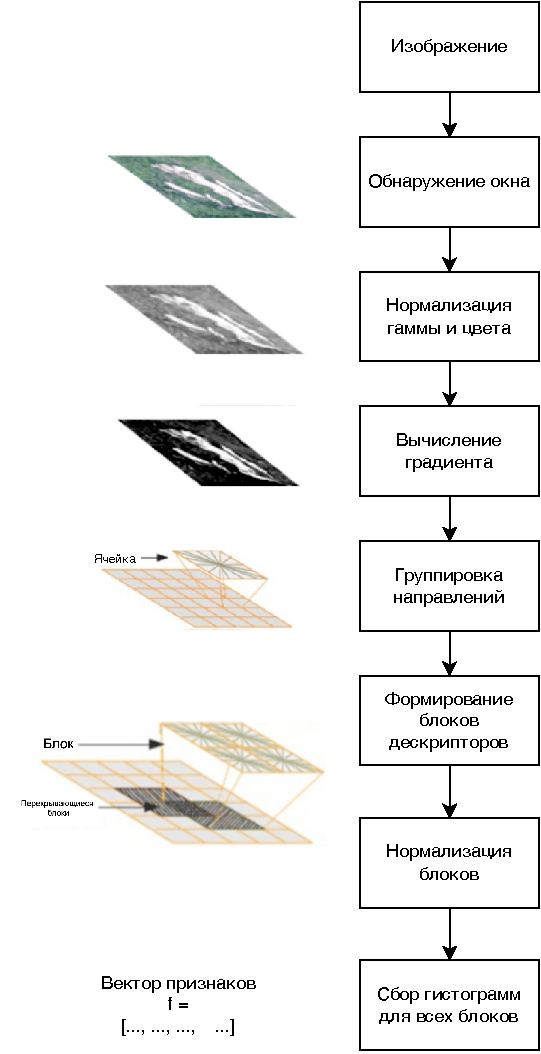
\includegraphics[width=0.7\textwidth]{img/hog.pdf}
% 	\caption{Схема алгоритма HOG.}
% 	\label{fig:hog}
% \end{figure}

% \clearpage


Рассмотренный метод имеет ряд преимуществ и недостатков при решении задачи классификации изображений.

Преимущества:
\begin{itemize}[leftmargin=1.6\parindent, label*=---]
	\item не требуется обучение, так как хранит набор данных;
	\item адаптация к изменяющимся данным, поскольку алгоритм не требует повторного обучения;
	\item устойчивость к переобучению.
\end{itemize}

Недостатки:
\begin{itemize}[leftmargin=1.6\parindent, label*=---]
	\item высокая вычислительная сложность;
	\item зависимость от выбора метрики и количества соседей;
	\item требует сбора признаков.
\end{itemize}

\subsection{Методы на основе деревьев принятия решений}

Методы на основе деревьев принятия решений представляют собой алгоритмы классификации, которые основываются на принципе создания дерева, где каждый узел представляет собой решающее правило, а каждая ветвь -- возможный исход этого правила. В рамках задачи классификации изображений можно применить следующие методы.

\subsubsection*{Дерево принятия решений}

Дерево принятия решений (Decision Tree) -- это базовый метод, где каждый узел дерева представляет собой один из признаков изображения, а каждая ветвь -- пороговое значение этого признака. Классификация производится путем прохождения по дереву, начиная с корневого узла и переходя на следующий узел в зависимости от значения признака, пока не будет достигнут листовой узел, который представляет конечный класс.

Алгоритм простого дерева принятия решений.
\begin{itemize}[leftmargin=1.6\parindent]
	\item[1.] Выбор признака. Из множества признаков выбирается тот, который наилучшим образом разделяет данные на разные классы. Обычно используется мера неоднородности, такая как критерий Джини\cite{gini-index} или энтропия, для определения приоритетности выбора признака.
	\item[2.] Разделение узлов. Данные разделяются на две (или более) части на основе выбранного признака. Каждый раздел создает дочерний узел в дереве.
	\item[3.] Повторение процесса. Процесс выбора признака и разделения данных повторяется для каждого дочернего узла, пока не будет выполнен критерий останова (например, достигнута определенная глубина дерева или узлы содержат данные одного класса).
	\item[4.] Листовые узлы. Когда выполнен критерий останова, узлы становятся листьями и представляют собой окончательные классификации.
	\item[5.] Прогноз. При поступлении нового наблюдения оно проходит по дереву, используя значения его признаков, и попадает в соответствующий лист, предсказывая тем самым класс данного наблюдения.
\end{itemize}

Простое дерево принятия решений часто служит строительным блоком для более продвинутых ансамблевых методов, таких как случайные леса или градиентный бустинг. В ансамблевых методах несколько слабых обучаемых моделей, таких как простые деревья решений, обучаются на разном подмножестве данных и затем комбинируются для улучшенной предсказательной способности.


\subsubsection*{Случайный лес}
Алгоритм случайный лес (Random Forest) -- это ансамблевый метод машинного обучения, который используется для классификации, регрессии и других задач. Он строится на основе концепции, где множество деревьев решений объединяются для достижения более точных прогнозов.
\newpage

Алгоритм случайного леса.
\begin{itemize}[leftmargin=1.6\parindent]
	\item[1.] Выбор случайной подвыборки. Из общего набора данных случайным образом выбирается подмножество данных (с повторениями).
	\item[2.] Построение деревьев решений. Для каждой подвыборки строится отдельное дерево решений. Процесс построения дерева аналогичен алгоритму дерева решений.
	\item[3.] Голосование. Когда поступает новое наблюдение, оно проходит через все построенные деревья, и каждое дерево дает свой прогноз. Затем происходит голосование, и классификация определяется большин-\\ством голосов.
	\item[4.] Использование случайности. Random Forest внедряет случайность в процесс построения деревьев, что позволяет каждому дереву быть уникальным. Это помогает уменьшить переобучение и повысить обобщающую способность модели.
	\item[5.] Усреднение прогнозов. Поскольку Random Forest состоит из множества деревьев, его прогнозы усредняются, что обычно приводит к улучшению точности по сравнению с одним деревом решений.
\end{itemize}

Важно отметить, что Random Forest обладает рядом дополнительных преимуществ, таких как возможность оценки важности признаков и автоматическое управление переобучением. Кроме того, он позволяет эффективно обрабатывать большие объемы данных с высокой размерностью признаков.

Однако, существует несколько недостатков, связанных с Random Forest, таких как более высокое время обучения по сравнению с одним деревом решений, потребность в тщательной настройке гиперпараметров и сложность интерпретации по сравнению с одиночным деревом решений.

\subsubsection*{Градиентный бустинг}

Градиентный бустинг (Gradient Boosting) -- это метод машинного обучения, который используется для построения прогностических моделей, таких как регрессия и классификация. Он основан на комбинировании слабых алгоритмов обучения (например, деревьев решений) в композицию, которая обладает более высокой предсказательной способностью.

Алгоритм градиентного бустинга.
\begin{itemize}[leftmargin=1.6\parindent]
	\item[1.] Инициализация модели. Строится начальная модель, которая может быть, например, классом с наибольшим количеством экземпляров для задачи классификации.
	\item[2.] Вычисление остатков. Вычисление остатков или ошибок предсказания начальной модели для каждого обучающего примера. Эти остатки становятся новой целевой переменной для следующей модели.
	\item[3.] Обучение слабой модели. Эта модель пытается предсказать остатки, полученные на предыдущем шаге, обычно для этого используются деревья решений небольшой глубины.
	\item[4.] Вычисление коэффициента, на который мы будем умножать предсказания новой модели, чтобы получить более точное предсказание композиции. Этот коэффициент вычисляется с использованием градиентного спуска или другого оптимизационного метода.
	\item[5.] Обновление композиции моделей, путем добавления новой модели, умноженной на вычисленный коэффициент.
	\item[6.] Повторение шагов 2-5 пока не достигнем определенного критерия останова, такого как количество итераций или улучшение метрики качества.
\end{itemize}

Градиентный бустинг обладает высокой предсказательной способностью и способен автоматически отбирать признаки, однако он чувствителен к переобучению и требует тщательной настройки гиперпараметров.


\section{Сравнение методов классификации}
\subsection{Формулировка критериев сравнения методов классификации}
Для сравнения рассмотренных алгоритмов можно выделить следующие критерии.
\begin{itemize}[leftmargin=1.6\parindent]
	\item[1.] Автоматическое создание признаков: этот критерий обозначает, способен ли выбранный метод автоматически генерировать признаки из исходных данных, или же требуется вручную задавать признаки. Генерация означает процесс преобразования исходных данных в более усовершенствованный формат, который может улучшить эффективность анализа и классификации.
	\item[2.] Автоматическое извлечение признаков: относится к способности метода автоматически определять и использовать наиболее важные или релевантные аспекты данных для классификации.
	\item[3.] Устойчивость к шуму: означает способность метода справляться с \\ошибками, неточностями или нежелательной информацией в данных.
	\item[4.] Точность в сложных задачах классификации:  измеряет, насколько верно метод определяет классы в трудных или многоклассовых задачах.
	\item[5.] Обработка сложных признаков: оценивает, насколько эффективно метод может обрабатывать сложные признаки, такие как непрерывные, категорийные или временные.
\end{itemize}


\subsection{Сравнительный анализ методов классификации}
\subsubsection*{На основе глубоких нейронных сетей}
\begin{itemize}[leftmargin=1.6\parindent]
	\item[1.] Автоматическое создание/извлечение признаков: данные методы работают напрямую с изображениями, без необходимости создавать и извлекать признаки, это происходит автоматически.
	\item[2.] Устойчивость к шуму:  средняя, в сравнении с другими рассмотренными методами, так как шум может приводить к изменениям в распределении данных и переобучению.
	\item[3.] Точность в сложных задачах классификации: высокая, в сравнении с другими рассмотренными методами, это связано с их способностью автоматически выявлять и анализировать признаки на всех уровнях абстракций.
	\item[4.] Обработка сложных признаков: глубокие нейронные сети способны обрабатывать сложные признаки, так как они автоматически извлекают признаки на разных уровнях сложности.
\end{itemize}

\subsubsection*{На основе экземпляров}
\begin{itemize}[leftmargin=1.6\parindent]
	\item[1.] Автоматическое создание/извлечение признаков: зависят от  разработанных и извлеченных человеком признаков для обучения.
	\item[2.] Устойчивость к шуму: сравнительно низкая, поскольку данные методы  зависят от близости измерений между точками данных.
	\item[3.] Точность в сложных задачах классификации: средняя, в силу того, что могут возникнуть трудности в случаях, когда классы не могут быть легко разделены в пространстве признаков.
	\item[4.] Обработка сложных признаков: данный метод имеет малую точность на больших объемами данных и низким уровнем сигнала, которые обычно связаны со сложными признаками.
\end{itemize}

\subsubsection*{На основе деревьев принятия решений}
\begin{itemize}[leftmargin=1.6\parindent]
	\item[1.] Автоматическое создание/извлечение признаков: зависят от разработанных и извлеченных человеком признаков для обучения.
	\item[2.] Устойчивость к шуму: сравнительно высокая,  поскольку данные методы делают предположения о структуре данных и не полагаются на расстояние между точками данных для классификации.
	\item[3.] Точность в сложных задачах классификации:  средняя, методы на основе деревьев принятия решений имеют сравнимую точность с методами на основе экземпляров, но уступают методам на основе глубоких нейронных сетей.
	\item[4.] Обработка сложных признаков: обычные деревья принятия решений, как правило, не очень хорошо справляются с  сложными признаками, потому что их стратегия разделения может привести к переобучению. Однако более современные алгоритмы, такие как случайные леса и градиентный бустинг, могут выполнять иерархическое или несколько уровневое разбиение, что позволяет им лучше справляться со сложной структурой данных.
\end{itemize}


Сравнительная характеристика рассмотренных методов представлена в таблице \ref{tab:comp-methods}.

\begin{table}[h]
	\centering
	\setlength{\extrarowheight}{-5pt}
	\caption{Таблица сравнение методов.}
	\label{tab:comp-methods}
	\begin{tabular}{|c|c|c|c|}
		\hline
		Метод                                                                                  & \begin{tabular}[c]{@{}c@{}} \cellcolor{blue!20} На основе \\ \cellcolor{blue!20} глубоких\\  \cellcolor{blue!20}нейронных сетей\end{tabular} & \begin{tabular}[c]{@{}c@{}}На основе \\ экземпляров\end{tabular} & \begin{tabular}[c]{@{}c@{}}На основе деревьев\\ принятия решений\end{tabular} \\ \hline
		\begin{tabular}[c]{@{}c@{}}Обработка \\ сложных \\ признаков\end{tabular}              & $+$                                                                                & $-$                                                                & $\pm$                                                                            \\ \hline
		\begin{tabular}[c]{@{}c@{}}Точность в сложных \\ задачах \\ классификации\end{tabular} & высокая                                                                          & средняя                                                          & средняя                                                                       \\ \hline
		\begin{tabular}[c]{@{}c@{}}Устойчивость\\ к шуму\end{tabular}                          & средняя                                                                          & низкая                                                           & высокая                                                                       \\ \hline
		\begin{tabular}[c]{@{}c@{}}Автоматическое \\ извлечение\\ признаков\end{tabular}       & $+$                                                                                & $-$                                                                & $-$                                                                             \\ \hline
		\begin{tabular}[c]{@{}c@{}}Автоматическое\\ создание\\ признаков\end{tabular}          & $+$                                                                                & $-$                                                                & $-$                                                                             \\ \hline
	\end{tabular}
\end{table}
